{
\newcommand{\eeps}{e_\epsilon}

\section{Suitable title}
Let $(x, \eeps)$ be a pair with distribution the same as the two
dimensional process from Observation \ref{obs:2d-proc}.

Our goal in this section is to prove the following theorem:
\begin{theorem}\label{thm:main1}
Under the previous notations, $\eeps(1) \to x(1)$ in probability
as $\epsilon \to 0$.
\end{theorem}

\newcommand{\radiussq}{\delta^2}
\newcommand{\radius}{\delta}
\newcommand{\twonorm}[1]{||#1||_2}

\newcommand{\twodproc}[1]{(x(#1), \eeps(#1))}

In order to prove this it will be easier to prove the following
stronger claim:
\begin{propos}\label{thm:main2}
For every $t\in[0,1]$ and every $\radius>0$
$$\ds \lim_{\epsilon \rightarrow 0}\P\left(\text{either } x(t)=\eeps(t)
\text{ or } \twonorm{\twodproc{t}} <\radius\right)=1$$
Equivalently, until time $1$, the two dimensional process $\twodproc{t}$
leaves the $\radius$ ball only through $(\frac{\radius}{\sqrt2},\frac{\radius}{\sqrt2})$ or through $-(\frac{\radius}{\sqrt2},\frac{\radius}{\sqrt2})$, with high probability.
\FIXME{}{I'm not completely comfortable with this equivalent
  definition.  It's informal, though it has a formal counterpart, and
  it doesn't seem immediate that the formal counterpart is equivalent
  to Proposition \ref{thm:main2} -- Tom}
\end{propos}

We begin by presenting a handy property whose proof
we delay to Subsection \ref{sec:POC}:

\begin{propos}\label{thm:no-escape}
Suppose that at time $t_0$ we have
$\twodproc{t_0}=(0,0)$, let $t>0$ be the first time at which
$\twonorm{\twodproc{t}}=1$, then the probability
that $\twodproc{t} \not=\pm(\frac{1}{\sqrt2},\frac{1}{\sqrt2})$ is $O(\frac1{\log\epsilon})$.
\end{propos}

Applying scaling invariance to this theorem immediately yields the
following corollary:
\begin{cor}\label{cor:cor1}
Let $\radius>0$ suppose that at time $t_0$ we have $\twodproc{t_0}=(0,0)$, let
$t>0$ be the first time at which
$\twonorm{\twodproc{t}} = \radius$, then the probability
that $\twodproc{t} \not=\pm(\frac{\radius}{\sqrt2},\frac{\radius}{\sqrt2})$ is
$O(\frac{1}{\log\epsilon/\radiussq})$.
\end{cor}

In order to overcome the gap between Corollary \ref{cor:cor1} and
Theorem \ref{thm:main1} we quote without proof the following property of Brownian
motion:
\begin{propos}\label{prop:prop1}
Let $\zeta>0$ and let $x(t)$ be a one dimensional Brownian
motion such that $x(0)=0$. There exist some $k$ such that
$\P(\ds\sup_{t\in[0,1]}x(t)>k) <\zeta$.
\end{propos}

We are now ready to give a proof to Proposition \ref{thm:main2}.

\begin{proof}[Proof (Proposition \ref{thm:main2})]
\newcommand{\hitradius}[1]{\twonorm{\twodproc{#1}}=\radius}

Let us think of $b(t)=\twodproc{t}$ as a process which dies if ever $x(t)\neq\eeps(t)
\text{ or } \twonorm{\twodproc{t}} = \radius$.

We define a one-dimensional "$\radius$-Teleporting" Brownian motion: $x^{\radius}(t)$
 as a Brownian motion such that whenever it hits $0$ it teleports to $\frac1{\sqrt{2}}\radius$.
Proposition \ref{prop:prop1} implies that for all $\zeta>0$ there exists a $k$ such that the probability
that $x^{\radius}(t)$ is teleported more then $k$ times between times $0$ and $1$ is less then $\zeta$. Let $x^{\radius}(t)$ be such a teleporting Brownian motion, and let
 $d_i(t)=\twodproc{t}_i$ be an infinite sequence
 of independent random walks identical in distribution to $b(t)$, starting from $(0,0)$, such that each
 of them dies when $\twonorm{\twodproc{t}} = \radius$. We can now couple $b(t)$ with the set $\{x^\radius(t)\}\ds\bigcup_{i=1}^\infty\{d_i(t)\}$ in the following way:

Set $t_0=0$. We begin by coupling $d_1(t)$ with $b(t)$ until $d_1(t)$ terminates at 
time $t'_0$, if $x(t'_0)\neq\eeps(t'_0)$ then $b(t)$ terminates as well, otherwise
 if $x(t_0)=\frac1{\sqrt{2}}\radius$ we couple $b(t)$ with $(\frac{x^\radius(t-t'_0+t_0)}{\sqrt{2}},\frac{x^\radius(t-t'_0+t_0)}{\sqrt{2}})$,
  and if $x(t_0)=-\radius$ we couple $b(t)$ with $-(\frac{x^\radius(t-t'_0+t_0)}{\sqrt{2}},\frac{x^\radius(t-t'_0+t_0)}{\sqrt{2}})$.
 This continues until time $t_1$, the first to satisfy $b(t_1)=(0,0)$ after $t'_0$, 
 at which we couple $b(t)$ with $d_2(t-t_1)$, and so on and so forth.

Let us look at the event that $x^\radius(t)$ has teleported at most $k$ times by time $1$.
 By Proposition \ref{prop:prop1} we can pick $k$ such that this probability will be as small 
 as we want. The events that $d_i$ for $i\le k$ terminated on a point such that $x=\eeps$ 
 are independent and by Corollary \ref{cor:cor1} can be made as small as we want. However
  if both events do not occur - the coupling insures us that by time $t=1$ the two
   dimensional process $b(t)$
leaves the $\radius$ ball only through
$\frac1{\sqrt2}(\radius,\radius)$ or through
$\frac1{\sqrt2}(-\radius,-\radius)$. We deduce that the two dimensional process $b(t)=\twodproc{t}$
a.s.\ leaves the $\radius$ ball only through $(\frac{\radius}{\sqrt2},\frac{\radius}{\sqrt2})$ or through $-(\frac{\radius}{\sqrt2},\frac{\radius}{\sqrt2})$.

\end{proof}

\subsection{Proof of convergence}\label{sec:POC}
{
%Let $\xi_\epsilon=(X,Y,\epsilon)$ as before. We denoted by $\eeps(t)$ a sample of $\xi_\epsilon$
%starting at some given point at time $0$. We also denote by $x(t)$ a
%sample of $X$ starting at the same point.
%NB: \xi no longer exists above -- Tom
In this section we prove Proposition \ref{thm:no-escape}. Our main technical tool in doing so will
be conformal maps. We begin by rotating the process $\twodproc{\cdot}$
through $\pi/4$ radians clockwise about the origin to get a process
$b_\epsilon(t)$ \FIXME{which is absorbing only along the \FIXME{$x$
    axis}{$x$ is a constant in earlier notation}}{this is a note to
  make it clearer to the reader exactly what's going on, but perhaps
  it should be clearer}.
Sometimes, we will omit the $\epsilon$ writing $b(t)$. \FIXME{We always assume $\epsilon$
to be sufficiently small.}{This is a confusing statement.  What does
  it actually mean?  Are there actually any cases where this
  assumption is used?  If not, let's delete it -- Tom}
We can now rephrase Proposition
\ref{thm:no-escape} as:

\begin{propos}[Proposition \ref{thm:no-escape} rephrased]\label{prop:reph}
Suppose that at time $t_0$ we have
${b}(t_0)=(0,0)$, let $t_1>0$ be the first time at which
$||b(t_1)||_2=1$, then the probability that $b(t_1)\neq \pm(1,0)$ is
$O\left(\frac1{\log\epsilon}\right)$.
\end{propos}

We define the following indicator function
\newcommand{\online}[1]{A(#1)}
\[\online{t} := (b(t) \text{ is on the x axis and its x component has modulus
} > \epsilon)\]
Note that whenever $\online{t}=1$,
we can regard $b(t)$ as a one dimensional Brownian motion on the
$x$-axis, while whenever $\online{t}=0$ we can regard it as a two
dimensional Brownian motion. We can now treat the sampled
process $b_\epsilon(t)$ as a state machine with $4$ states
$a_0,a^r_1,a_{\text{win}},a_{\text{lose}}$, one of which ($a^r_1$) has a parameter $r$.

The states are defined in the following way:
\begin{enumerate}
\item\label{n1} $b_\epsilon(t)$ is in state $a_0$ whenever $\online{t}=0$.
\item\label{n2} $b_\epsilon(t)$ is in state $a^r_1$ whenever $\online{t}=1$ and $|x(\sup_{s<t}(\online{s}=0))|=r$.
\item\label{n3} $b_\epsilon(t)$ is in state $a_\text{win}$ whenever $b_\epsilon(t)=(1,0)$.
\item\label{n4} $b_\epsilon(t)$ is in state $a_\text{lose}$ whenever $b_\epsilon(t)\neq(1,0)$ yet $||b_\epsilon(t)||_2=1$.
\end{enumerate}

By this definition, at time $0$ our state machine is in state $a_0$.
We strive to prove that the probability to get to
 state $a_\text{lose}$ before getting to $a_\text{win}$ is $O(\frac1{\log\epsilon})$.
 We do this by calculating the transition functions of
 this state machine. This calculation is describe by the following proposition,
 while the state machine is depicted in Figure \ref{fig:state_machine}.

 \begin{figure}[htb]
\begin{center}
\leavevmode
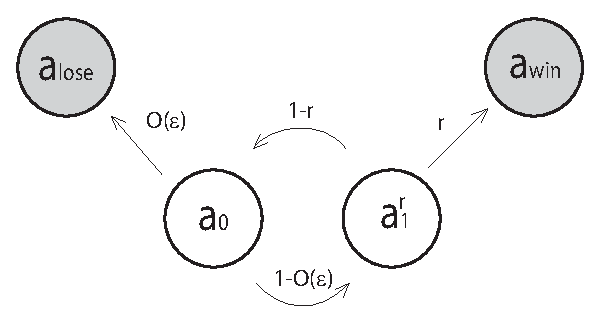
\includegraphics{state_machine.eps}
\end{center}
\caption{A diagram of the state machine.}
\label{fig:state_machine}
\end{figure}

\begin{propos}[Transition probabilities]\label{prop:trans}
The following is the transition probability of the state machine described above:
\begin{enumerate}
\item\label{m11} $\P(a^r_1\rightarrow a_0)=1-r$
\item\label{m12} $\P(a^r_1\rightarrow a_\text{win})=r$
\item\label{m13} $\P(a^r_1\rightarrow a_\text{lose})=0$
\item\label{m21} $\P(a_0\rightarrow a_\text{win})=0$
\item\label{m22} $\P(a_0\rightarrow a_\text{lose})=O(\epsilon)$
\item\label{m23} $\P(a_0\rightarrow a^r_1 \text{ for some }r)=1-O(\epsilon)$
\item\label{m24} $\P(a_0\rightarrow a^r_1 \text{ such that } r_0<r<r_1)>\ds c\epsilon\left(\frac 1 {r_0}-\frac 1 {r_1}-1\right)$ for $r_0>2\epsilon$.
%$\P(a_0\rightarrow a^r_1 \text{ such that } r_0<r<r_1)>\ds\int_{r_0}^{r_1}(\frac{c\epsilon}{r^2}-0.5)dr$ for $r_0>2\epsilon$
\end{enumerate}
$a_\text{win}$ and $a_\text{lose}$ are trap states which are assigned no transition function.
\end{propos}

\begin{proof}
 On $a^r_1$ we know $b(t)$ is a $1$-dimensional Brownian motion starting at $r$.
 We can treat the transition time of $b(t)$ from $a^r_1$ to either $a_0$ or
 $a_\text{win}$ as a stopping time for such a Browinian motion, getting
 \ref{m11} and \ref{m12} immediately. The definition of the different states
 implies \ref{m13} and \ref{m21}. The proofs of \ref{m22}, \ref{m23} and \ref{m24}
 are given separately in Corollaries \ref{m22and23true} and \ref{m24true} in Section \ref{sec:ROI}.
\end{proof}

Analyzing the transition probabilities described in Proposition \ref{prop:trans} we
can find the probability of reaching $a_\text{lose}$ before $a_\text{win}$ and vice versa.
 The main step towards this result is the following proposition:

\begin{propos}\label{prop:winlose1}
Let $s_1=a_0,...,s_n$ be the sequence of states of our state machine.
\begin{equation}\label{eq:losecase}
\P(s_n=a_\text{lose} \text{ and } \ds\forall_{i>1}(s_i\neq a_0))=O(\epsilon)
\end{equation}
\begin{equation}\label{eq:wincase}
\P(s_n=a_\text{win} \text{ and } \ds\forall_{i>1}(s_i\neq a_0))=\Omega(\epsilon\log\epsilon)
\end{equation}
\end{propos}

\begin{proof}
Both \eqref{eq:losecase} and \eqref{eq:wincase} are direct results of Proposition \ref{prop:trans}.
 $a_0$ can be followed only by $a_\text{lose}$ and $a_1^r$. However $a_\text{lose}$ cannot be
 reached from $a_1^r$ without passing through
 $a_\text{win}$, thus:
 $$\P(s_n=a_\text{lose} \text{ and } \ds\forall_{i>1}(s_i\neq a_0))=\P(a_0\rightarrow a_\text{lose})=O(\epsilon)$$
 where the last equality is by item \ref{m22} in Proposition \ref{prop:trans}.
 This concludes the proof of \eqref{eq:losecase}.

 In order to reach $a_\text{win}$ from $a_0$, we must have $a_1^r$ following $a_0$, and then $a_\text{win}$
  following $a_1^r$. By Fubini's Theorem, this yields the following formula:
 \begin{equation}\label{eq:r1}
 \P(s_n=a_\text{win} \text{ and } \ds\forall_{i>1}(s_i\neq a_0))=\ds\int_{\epsilon}^1 f(r) \P(a^r_1\rightarrow a_\text{win}) dr
 \end{equation}
 Where $f(r)$ is the density of the random variable $r$ which gets $r$ when
 $a_0\rightarrow a^r_1$ and $0$ otherwise. Since the density of a random variable is non-negative, we get:
 \begin{equation}\label{eq:r2}
 \P(s_n=a_\text{win} \text{ and } \ds\forall_{i>1}(s_i\neq a_0))\ge\ds\int_{2\epsilon}^1 f(r) \P(a^r_1\rightarrow a_\text{win}) dr
 \end{equation}
Applying items \ref{m24} and \ref{m12} of Proposition \ref{prop:trans} to \eqref{eq:r2}, we get:
\begin{equation}\label{eq:r3}
 \P(s_n=a_\text{win} \text{ and } \ds\forall_{i>1}(s_i\neq a_0))\ge \ds\int_{2\epsilon}^1 c\epsilon\left(\frac{1}{r^2}-1\right)r\, dr = \Omega(\epsilon\log\epsilon).
\end{equation}
\end{proof}

Proposition \ref{prop:reph} is an immediate consequence of Proposition
\ref{prop:winlose1}. Indeed, suppose that at time $t_0$ we have
$e(t_0)=0$, let $t_1>t_0$ be the first time at which $||b(t_1)||_2=1$.
By Proposition \ref{prop:winlose1} we have
$$\frac{\P (y(t_1)\neq0)}{\P (y(t_1)=0)}=O\left(\frac 1 {\log\epsilon}\right).$$
}

\subsection{Results on Integrals}\label{sec:ROI}

The main goal of this subsection is to prove items \ref{m22} - \ref{m24} in Proposition
 \ref{prop:trans}. In order to understand the proofs of those items and the link
  between them, we should refer once more to the process described in the
   beginning of Section \ref{sec:POC}. When one wishes to estimate the
   transition probabilities from state $a_0$ in our state machine, one
   actually inquires about the behavior of a complex Brownian motion in
   the domain $D=\{||x||<1\}\setminus\{|\Re x|>\epsilon,\,\Im y=0\}$. This
   process terminates when it hits the boundary of the domain. Let us
   denote such a process $B(t)=(x(t),y(t))$. We will use a conformal
    map $\phi$ to map $D$ to the unit ball $\{||x||<1\}$ such that
    under $\phi$ we have $-i \mapsto-i$, $i\mapsto i$ and
    $\epsilon\mapsto-1$. Since those are three points on the
     boundary of $D$ they define a unique conformal map from it
      to the unit disk \TODO{}{write a reference?}. By symmetry
      this also implies $0\mapsto0$, $-i\mapsto -i$, and
       $-\epsilon\mapsto1$. The conformal map $\phi$ is
       illustrated in Figure \ref{fig:conf_map}.
\begin{figure}[htb]
\begin{center}
\leavevmode
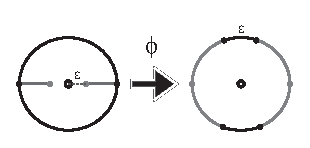
\includegraphics{conformal_map.eps}
\end{center}
\caption{The conformal map $\phi$ from $D$ to the unit circle}
\label{fig:conf_map}
\end{figure}

Our main result of this subsection is:
\begin{propos}\label{prop:confmain}
The conformal map above has:
$$\Re \phi(z) = -\frac{\epsilon}{1+\epsilon^2}\frac{1+z^2}{z},$$
for $z\in\mathbb{R}$ such that $\epsilon\le|z|\le1$.
\end{propos}
\begin{proof}
The main instrument in our proof is the explicit description of $\phi$.
We ease this description on the reader, by describing two
auxiliary functions, $G(z)$ and $H(z)$. We define $G(z)=\frac{1+z}{1-z}$
and $H(z)=\frac1{g(z)^2+g(-\epsilon)^2}$. We then define
\begin{equation}\label{eq:functionf}
\phi(z)=\frac{i\sqrt{H(\epsilon)-H(z)}-\sqrt{H(0)-H(\epsilon)}}{i\sqrt{H(\epsilon)-H(z)}+\sqrt{H(0)-H(\epsilon)}}
\end{equation}
\TODO{}{should we show that $\phi(z)$ is indeed the conformal map we are after?}
We can multiply \eqref{eq:functionf} by its numerator to calculate $\Re \phi(x)$, when $x$ is real. This calculation yields
\begin{equation}\label{eq:refunctionf}
\Re \phi(z)=\frac{H(0)-2H(\epsilon)+H(z)}{H(0)-H(T)}
\end{equation}
Expanding \eqref{eq:refunctionf}, and using the fact $\epsilon\le |z|\le1$ we get:
$\Re \phi(z) = -\frac{\epsilon}{1+\epsilon^2}\frac{1+z^2}{z}$ as required.
\end{proof}

The next couple of Corollaries will establish the unresolved parts of Proposition \ref{prop:trans}. Both will use the fact a Brownian motion has radial symmetry in the plane and thus its chance of leaving a circle through some arc is proportional to its length.

\begin{cor}\label{m22and23true}
Items \ref{m22} and \ref{m23} in Proposition \ref{prop:trans} are true.
\end{cor}
\begin{proof}
Denote by $u$ the length of each of the two arcs in the unit circle which are the images of the arcs $1\frown-1$. By Proposition \ref{prop:confmain} we have $\Re \phi(-1)=-\Re \phi(1)=2\frac{\epsilon}{1+\epsilon^2}$. As the length of an arc in a semicircle cannot exceed $\pi$ times the length of a string leaning on it, we get $u<\frac{4\pi\epsilon}{1+\epsilon^2}<O(\epsilon)$.
\end{proof}

\begin{cor}\label{m24true}
Item \ref{m24} in Proposition \ref{prop:trans} is true.
\end{cor}
\begin{proof}

In order to prove Item \ref{m24} in Proposition \ref{prop:trans}, we should calculate the length $u$ of the arc between $\phi(-r_0)$ and $\phi(-r_1)$.
%By Proposition \ref{prop:confmain} we have $\Re\phi(-r_i)=\frac{\epsilon}{1+\epsilon^2}\frac{1+r_i^2}{r_i}$ for $i\in\{0,1\}$.
%Since $r_0>2\epsilon$,
%$|\Re\phi(-r_1)-\Re\phi(-r_0)| \frac{\Re \phi (2\epsilon)}{ \sqrt {1-\Re \phi (2\epsilon)^2}} \le u$.

Notice that $\phi(r)$ lies on a semi-circle for $r\in[2\epsilon,1]$, and that the slope of the semicircle is bounded from below (say by $m$) on $\Re\phi([2\epsilon,1])$. This leads to the bound: $|\Re\phi(-r_1)-\Re\phi(-r_0)| m \le u$.
On the other hand,
$$|\Re\phi(-r_1)-\Re\phi(-r_0)|=\frac{\epsilon}{1+\epsilon^2}\left|\frac{1+r_1^2}{r_1}-\frac{1+r_0^2}{r_0}\right|\ge\epsilon\left(\frac 1 {r_0} - \frac 1{r_1}-1 \right). $$

\end{proof}




}
